\documentclass{ximera}  


%\usepackage{todonotes}
%\usepackage{mathtools} %% Required for wide table Curl and Greens
%\usepackage{cuted} %% Required for wide table Curl and Greens
\newcommand{\todo}{}

\usepackage{esint} % for \oiint
\ifxake%%https://math.meta.stackexchange.com/questions/9973/how-do-you-render-a-closed-surface-double-integral
\renewcommand{\oiint}{{\large\bigcirc}\kern-1.56em\iint}
\fi


\graphicspath{
  {./}
  {jpg}
  {ximeraTutorial/}
  {basicPhilosophy/}
  {functionsOfSeveralVariables/}
  {normalVectors/}
  {lagrangeMultipliers/}
  {vectorFields/}
  {greensTheorem/}
  {shapeOfThingsToCome/}
  {dotProducts/}
  {partialDerivativesAndTheGradientVector/}
  {../productAndQuotientRules/exercises/}
  {../motionAndPathsInSpace/exercises/}
  {../normalVectors/exercisesParametricPlots/}
  {../continuityOfFunctionsOfSeveralVariables/exercises/}
  {../partialDerivativesAndTheGradientVector/exercises/}
  {../directionalDerivativeAndChainRule/exercises/}
  {../commonCoordinates/exercisesCylindricalCoordinates/}
  {../commonCoordinates/exercisesSphericalCoordinates/}
  {../greensTheorem/exercisesCurlAndLineIntegrals/}
  {../greensTheorem/exercisesDivergenceAndLineIntegrals/}
  {../shapeOfThingsToCome/exercisesDivergenceTheorem/}
  {../greensTheorem/}
  {../shapeOfThingsToCome/}
  {../separableDifferentialEquations/exercises/}
  {vectorFields/}
}

\newcommand{\mooculus}{\textsf{\textbf{MOOC}\textnormal{\textsf{ULUS}}}}

\usepackage{tkz-euclide}\usepackage{tikz}
\usepackage{tikz-cd}
\usetikzlibrary{arrows}
\tikzset{>=stealth,commutative diagrams/.cd,
  arrow style=tikz,diagrams={>=stealth}} %% cool arrow head
\tikzset{shorten <>/.style={ shorten >=#1, shorten <=#1 } } %% allows shorter vectors

\usetikzlibrary{backgrounds} %% for boxes around graphs
\usetikzlibrary{shapes,positioning}  %% Clouds and stars
\usetikzlibrary{matrix} %% for matrix
\usepgfplotslibrary{polar} %% for polar plots
\usepgfplotslibrary{fillbetween} %% to shade area between curves in TikZ
\usetkzobj{all}
\usepackage[makeroom]{cancel} %% for strike outs
%\usepackage{mathtools} %% for pretty underbrace % Breaks Ximera
%\usepackage{multicol}
\usepackage{pgffor} %% required for integral for loops



%% http://tex.stackexchange.com/questions/66490/drawing-a-tikz-arc-specifying-the-center
%% Draws beach ball
\tikzset{pics/carc/.style args={#1:#2:#3}{code={\draw[pic actions] (#1:#3) arc(#1:#2:#3);}}}



\usepackage{array}
\setlength{\extrarowheight}{+.1cm}
\newdimen\digitwidth
\settowidth\digitwidth{9}
\def\divrule#1#2{
\noalign{\moveright#1\digitwidth
\vbox{\hrule width#2\digitwidth}}}





\newcommand{\RR}{\mathbb R}
\newcommand{\R}{\mathbb R}
\newcommand{\N}{\mathbb N}
\newcommand{\Z}{\mathbb Z}

\newcommand{\sagemath}{\textsf{SageMath}}


%\renewcommand{\d}{\,d\!}
\renewcommand{\d}{\mathop{}\!d}
\newcommand{\dd}[2][]{\frac{\d #1}{\d #2}}
\newcommand{\pp}[2][]{\frac{\partial #1}{\partial #2}}
\renewcommand{\l}{\ell}
\newcommand{\ddx}{\frac{d}{\d x}}

\newcommand{\zeroOverZero}{\ensuremath{\boldsymbol{\tfrac{0}{0}}}}
\newcommand{\inftyOverInfty}{\ensuremath{\boldsymbol{\tfrac{\infty}{\infty}}}}
\newcommand{\zeroOverInfty}{\ensuremath{\boldsymbol{\tfrac{0}{\infty}}}}
\newcommand{\zeroTimesInfty}{\ensuremath{\small\boldsymbol{0\cdot \infty}}}
\newcommand{\inftyMinusInfty}{\ensuremath{\small\boldsymbol{\infty - \infty}}}
\newcommand{\oneToInfty}{\ensuremath{\boldsymbol{1^\infty}}}
\newcommand{\zeroToZero}{\ensuremath{\boldsymbol{0^0}}}
\newcommand{\inftyToZero}{\ensuremath{\boldsymbol{\infty^0}}}



\newcommand{\numOverZero}{\ensuremath{\boldsymbol{\tfrac{\#}{0}}}}
\newcommand{\dfn}{\textbf}
%\newcommand{\unit}{\,\mathrm}
\newcommand{\unit}{\mathop{}\!\mathrm}
\newcommand{\eval}[1]{\bigg[ #1 \bigg]}
\newcommand{\seq}[1]{\left( #1 \right)}
\renewcommand{\epsilon}{\varepsilon}
\renewcommand{\phi}{\varphi}


\renewcommand{\iff}{\Leftrightarrow}

\DeclareMathOperator{\arccot}{arccot}
\DeclareMathOperator{\arcsec}{arcsec}
\DeclareMathOperator{\arccsc}{arccsc}
\DeclareMathOperator{\si}{Si}
\DeclareMathOperator{\scal}{scal}
\DeclareMathOperator{\sign}{sign}


%% \newcommand{\tightoverset}[2]{% for arrow vec
%%   \mathop{#2}\limits^{\vbox to -.5ex{\kern-0.75ex\hbox{$#1$}\vss}}}
\newcommand{\arrowvec}[1]{{\overset{\rightharpoonup}{#1}}}
%\renewcommand{\vec}[1]{\arrowvec{\mathbf{#1}}}
\renewcommand{\vec}[1]{{\overset{\boldsymbol{\rightharpoonup}}{\mathbf{#1}}}\hspace{0in}}

\newcommand{\point}[1]{\left(#1\right)} %this allows \vector{ to be changed to \vector{ with a quick find and replace
\newcommand{\pt}[1]{\mathbf{#1}} %this allows \vec{ to be changed to \vec{ with a quick find and replace
\newcommand{\Lim}[2]{\lim_{\point{#1} \to \point{#2}}} %Bart, I changed this to point since I want to use it.  It runs through both of the exercise and exerciseE files in limits section, which is why it was in each document to start with.

\DeclareMathOperator{\proj}{\mathbf{proj}}
\newcommand{\veci}{{\boldsymbol{\hat{\imath}}}}
\newcommand{\vecj}{{\boldsymbol{\hat{\jmath}}}}
\newcommand{\veck}{{\boldsymbol{\hat{k}}}}
\newcommand{\vecl}{\vec{\boldsymbol{\l}}}
\newcommand{\uvec}[1]{\mathbf{\hat{#1}}}
\newcommand{\utan}{\mathbf{\hat{t}}}
\newcommand{\unormal}{\mathbf{\hat{n}}}
\newcommand{\ubinormal}{\mathbf{\hat{b}}}

\newcommand{\dotp}{\bullet}
\newcommand{\cross}{\boldsymbol\times}
\newcommand{\grad}{\boldsymbol\nabla}
\newcommand{\divergence}{\grad\dotp}
\newcommand{\curl}{\grad\cross}
%\DeclareMathOperator{\divergence}{divergence}
%\DeclareMathOperator{\curl}[1]{\grad\cross #1}
\newcommand{\lto}{\mathop{\longrightarrow\,}\limits}

\renewcommand{\bar}{\overline}

\colorlet{textColor}{black}
\colorlet{background}{white}
\colorlet{penColor}{blue!50!black} % Color of a curve in a plot
\colorlet{penColor2}{red!50!black}% Color of a curve in a plot
\colorlet{penColor3}{red!50!blue} % Color of a curve in a plot
\colorlet{penColor4}{green!50!black} % Color of a curve in a plot
\colorlet{penColor5}{orange!80!black} % Color of a curve in a plot
\colorlet{penColor6}{yellow!70!black} % Color of a curve in a plot
\colorlet{fill1}{penColor!20} % Color of fill in a plot
\colorlet{fill2}{penColor2!20} % Color of fill in a plot
\colorlet{fillp}{fill1} % Color of positive area
\colorlet{filln}{penColor2!20} % Color of negative area
\colorlet{fill3}{penColor3!20} % Fill
\colorlet{fill4}{penColor4!20} % Fill
\colorlet{fill5}{penColor5!20} % Fill
\colorlet{gridColor}{gray!50} % Color of grid in a plot

\newcommand{\surfaceColor}{violet}
\newcommand{\surfaceColorTwo}{redyellow}
\newcommand{\sliceColor}{greenyellow}




\pgfmathdeclarefunction{gauss}{2}{% gives gaussian
  \pgfmathparse{1/(#2*sqrt(2*pi))*exp(-((x-#1)^2)/(2*#2^2))}%
}


%%%%%%%%%%%%%
%% Vectors
%%%%%%%%%%%%%

%% Simple horiz vectors
\renewcommand{\vector}[1]{\left\langle #1\right\rangle}


%% %% Complex Horiz Vectors with angle brackets
%% \makeatletter
%% \renewcommand{\vector}[2][ , ]{\left\langle%
%%   \def\nextitem{\def\nextitem{#1}}%
%%   \@for \el:=#2\do{\nextitem\el}\right\rangle%
%% }
%% \makeatother

%% %% Vertical Vectors
%% \def\vector#1{\begin{bmatrix}\vecListA#1,,\end{bmatrix}}
%% \def\vecListA#1,{\if,#1,\else #1\cr \expandafter \vecListA \fi}

%%%%%%%%%%%%%
%% End of vectors
%%%%%%%%%%%%%

%\newcommand{\fullwidth}{}
%\newcommand{\normalwidth}{}



%% makes a snazzy t-chart for evaluating functions
%\newenvironment{tchart}{\rowcolors{2}{}{background!90!textColor}\array}{\endarray}

%%This is to help with formatting on future title pages.
\newenvironment{sectionOutcomes}{}{}



%% Flowchart stuff
%\tikzstyle{startstop} = [rectangle, rounded corners, minimum width=3cm, minimum height=1cm,text centered, draw=black]
%\tikzstyle{question} = [rectangle, minimum width=3cm, minimum height=1cm, text centered, draw=black]
%\tikzstyle{decision} = [trapezium, trapezium left angle=70, trapezium right angle=110, minimum width=3cm, minimum height=1cm, text centered, draw=black]
%\tikzstyle{question} = [rectangle, rounded corners, minimum width=3cm, minimum height=1cm,text centered, draw=black]
%\tikzstyle{process} = [rectangle, minimum width=3cm, minimum height=1cm, text centered, draw=black]
%\tikzstyle{decision} = [trapezium, trapezium left angle=70, trapezium right angle=110, minimum width=3cm, minimum height=1cm, text centered, draw=black]




 
\title{Kirchoff's Laws} 
\author{Milica Markovic} 
\outcome{Apply phasor transformation to Kirchoff's Laws.}
\begin{document}  
\begin{abstract}  
Phasors are essential tool in circuit analysis.
\end{abstract}  
\maketitle    



In this section, we apply the phasor transformation to an RC circuit shown in Figure 2\ref{RCcirc}.  To solve this circuit in the time domain, we apply Kirchoff's voltage law, as shown in Equation \ref{eq-1} -\ref{eq0}.


The circuit in Figure \ref{RCcirc} is a simple RC circuit.  Equation \ref{eq-1} shows the KVL the time domain.

\begin{eqnarray}
        v_s(t)=v_R(t)+v_C(t)                \label{eq-1}  \\
v_s(t) = R i + \frac{1}{C} \int i(t) dt \label{eq0}
\end{eqnarray} 


As we discussed in the previous section, we will be using the principle of superposition, and add another generator to the circuit, as shown in Figure \ref{RCcirc}.

\begin{figure}[htbp]
\begin{center}
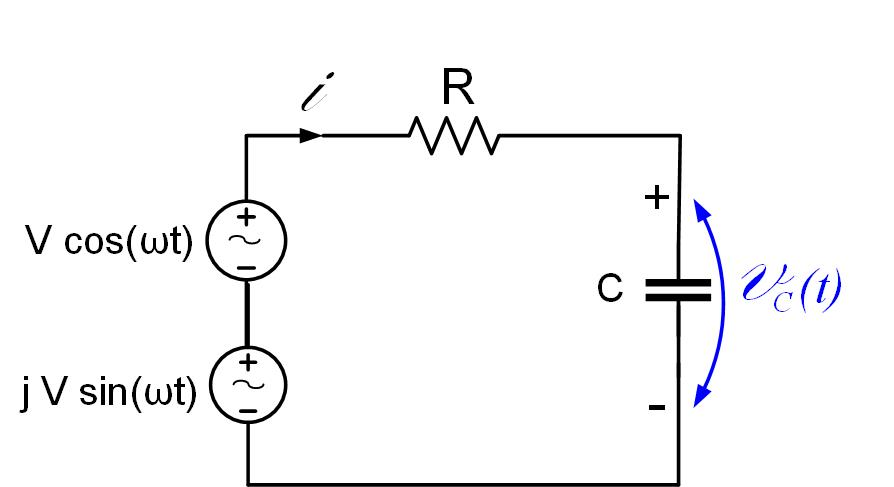
\includegraphics[scale=0.5]{../jpg/RCcircuitPhasorSup.jpg}
%\strut\psfig{figure=complexnumberz.ps,width=3cm} \\
\end{center}
\caption{Using superposition to find phasors of voltages and currents in an RC circuit.}
\label{RCcirc}
\end{figure}

The generator we originally had in the circuit is now just the real part of the phasor expression shown in Equation \ref{eq2}.


\begin{eqnarray}
v_s(t)=  V \cos (\omega t + \Theta_V)=\Re\{ V cos (\omega t + \Theta ) + j V sin (\omega t + \Theta)\}= \nonumber \\ 
= \Re\{V e^{j(\omega t + \Theta)}\}=\Re\{V e^{j \Theta} e^{j \omega t}\} \label{eq2}
\end{eqnarray}
We can now use the analysis from the previous section to  replace the time-domain quantities in equation \ref{eq0} with
these newly developed expressions.



\begin{eqnarray}
v_s(t)=v_R(t) + v_C(t)  \\
Re\{V_s e^{j \Theta_V} e^{j \omega t}\}=    \Re\{R \, I e^{j \Theta_I} e^{j \omega t}\}   +  \Re\{   \frac{1}{j \omega C}  I e^{j \Theta_I}  e^{j \omega t}  \}
\end{eqnarray}

A common term in the previous equation is $ e^{j\omega t}$, and we can now drop $Re$, as long as we later remember to take only the real part of the expression for the voltage and current phasors to get the time domain expression. We can now
write the equation as




\begin{eqnarray}
 V_s  e^{j \Theta_{V}}  =R \, I e^{j \Theta_I}  +    \frac{1}{j \omega C}  I e^{j \Theta_I}  \\
\tilde{V}_s  = R \tilde{I}    + \frac{\tilde{I}}{j \omega C} 
\end{eqnarray}



Since this is a linear equation, we can easily solve it:


\begin{eqnarray}
\tilde{I}  = \frac{\tilde{V}_s}{ R    + \frac{1}{j \omega C} } \label{pheq}
\end{eqnarray} 




\section{Converting the phasor back to the time domain}


In general, if the phasor is  $\tilde{V}=|V| e^{j \Theta_V}$, to find the time-domain signal, we first multiply the phasor with $e^{j \omega t}$ term, and then take the real part of it. 

\begin{eqnarray}
v(t)=\Re \{ \tilde{V} e^{j \omega t} \} \\
v(t)=\Re\{|\tilde{V}| e^{j(\omega t + \Theta_V)}\} \\
v(t)=\Re\{ |\tilde{V}| cos (\omega t + \Theta_V ) + j  |\tilde{V}|  sin (\omega t + \Theta_V)\} \\
v(t) = V cos (\omega t + \Theta_V )
\end{eqnarray}


\begin{example}
The phasor of current is  $I=3 e^{j 45^o}$. Obtain the signal in the time domain.


\begin{explanation}
  To obtain the time-domain signal from the phasor:
\begin{enumerate}
\item multiply the phasor $\tilde{I}$ with the $ e^{j\omega t}$ term, 
\item use Euler's formula 
\item take the real part of the expression.
\end{enumerate}  
   


\begin{eqnarray}
i(t) = \Re\{ 3 e^{ j 45^o}  e^{j\omega t} \} =  \Re\{3  e^{j \omega t + 45^o}  \} = \nonumber \\ = \Re \{ 3 \cos (\omega t + 45^o ) + j 3 \sin (\omega t + 45^o \} = 3  \cos (\omega t + 45^o ) \label{phtotd}
\end{eqnarray}


\end{explanation}


\end{example}


\begin{question}
The phasor for the  voltageis given as $\tilde{V}= 5 e^{ j \beta } $. Find the expression for the phasor in the time domain.
\begin{multipleChoice}  
\choice{$v(t) = 5 \cos \beta t $}  
\choice[correct]{$v(t) = 5 \cos (\omega t+ \beta)$}  
\choice{$v(t) = 5 \sin \beta t$}  
\end{multipleChoice} 
\end{question}

\end{document} 
